\section{Introduction}
Modeling is a powerful tool in synthetic biology. It provides us with a necessary engineering approach to characterize our pathways quantitatively and predict their performance, thus help us test and modify our design. Through the dynamic model of heavy-metal detection biosensor, we hope to gain insights into the characteristics of our whole circuit's dynamics.

\section{Methods}
\subsection{Analysis of metabolic pathways}
\begin{figure}[h]
	\centering
	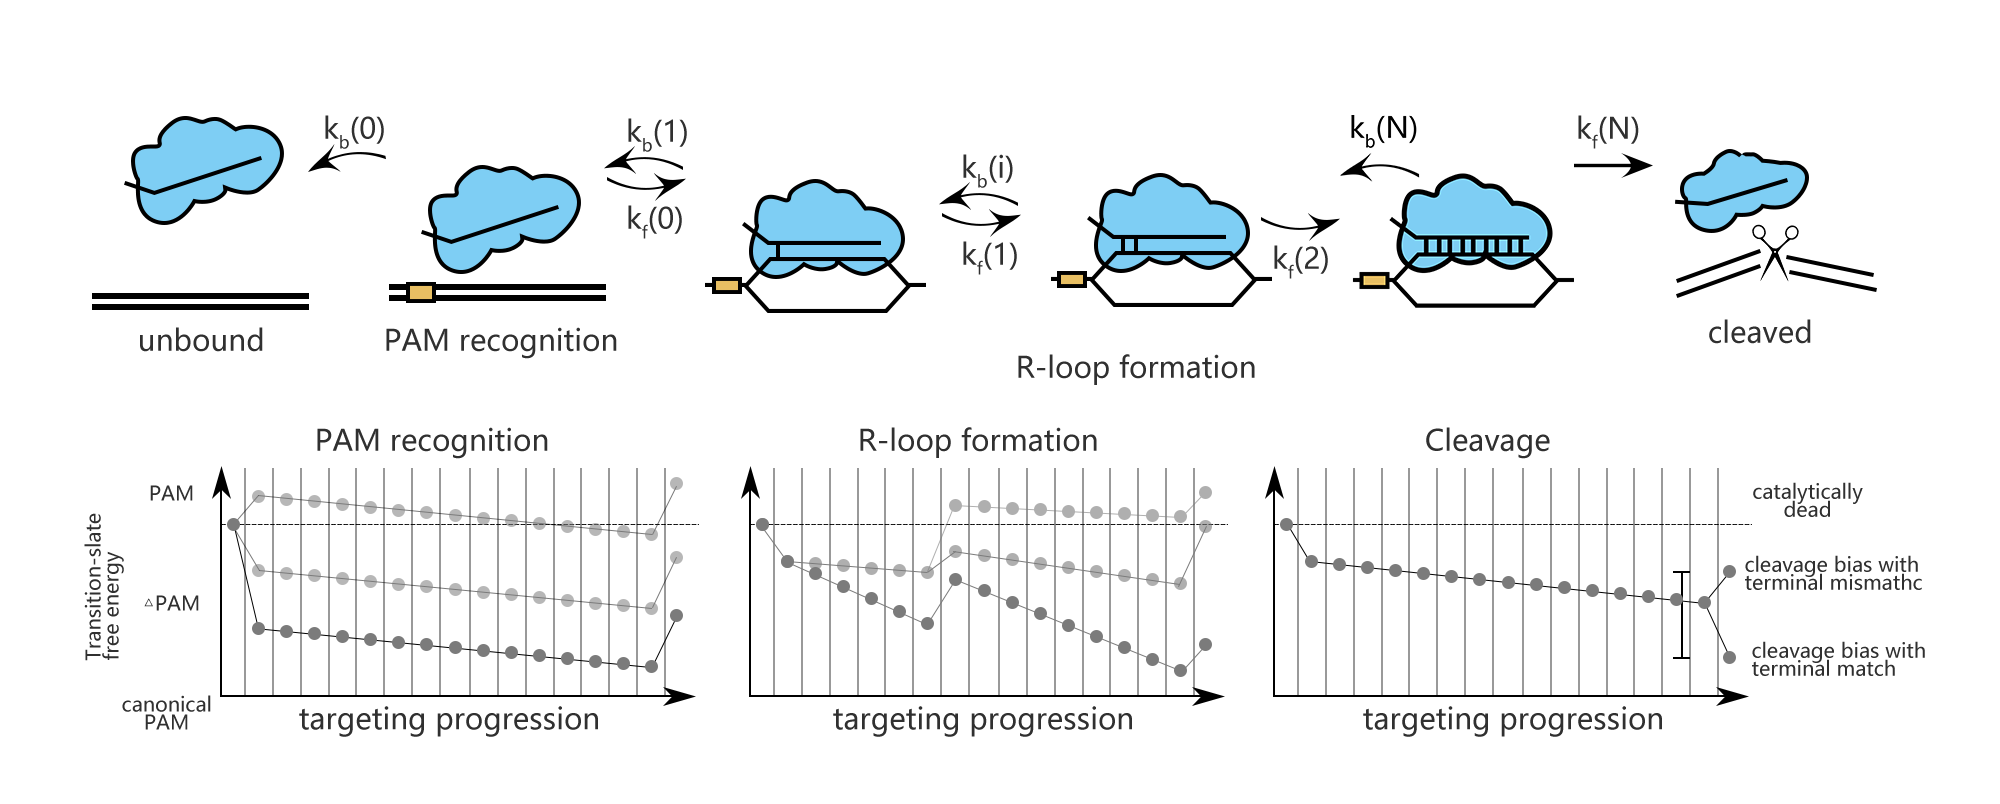
\includegraphics[width=12cm]{1}
	\caption{Metabolic pathways related to plasmid\#1}
\end{figure}

At the beginning, on the plasmid\#1, the promoter P\textsubscript{arsR} isn't bound with ArsR, thus it is active. ArsR and smURFP are transcribed and translated under the control of the promoters P\textsubscript{arsR\textsubscript{u}} and P\textsubscript{arsR\textsubscript{d}}, with subscript u and d representing upstream and downstream separately. The subscript l of smURFP in the equation means leaky expression without the expression of As\textsuperscript{3+}. As ArsR is expressed gradually, it will bind with the promoter P\textsubscript{arsR} and make it inactive. \cite{pola2018novel}

\begin{equation}
	P_{J23104} \stackrel{k_{tx1}}{\longrightarrow} P_{J23104}+mRNA_{ArsR}
\end{equation}
\begin{equation}
	mRNA_{ArsR}\stackrel{k_{tl1}}{\longrightarrow} mRNA_{ArsR}+ArsR
\end{equation}
\begin{equation}
	P_{arsR} \stackrel{k_{tx2}}{\longrightarrow} P_{arsR} +mRNA_{smURFP}
\end{equation}
\begin{equation}
	mRNA_{smURFP} \stackrel{k_{tl2}}{\longrightarrow} mRNA_{smURFP}+ smURFP
\end{equation}

\begin{equation}
	ArsR+P_{arsR} \xrightleftharpoons[k_{-b1}]{k_{b1}}ArsR*P_{arsR} 
\end{equation} 
On the plasmid\#2, the fusion protein of dCas9 and RNAP(RNA polymerase) are produced after transcription and translation, and $sgRNA$ is produced after transcription.


\begin{equation}
	P_{tet} \stackrel{k_{tx3}}{\longrightarrow} P_{tet} +mRNA_\text{dCas9-RNAP}
\end{equation}
\begin{equation}
	mRNA_\text{dCas9-RNAP} \stackrel{k_{tl3}}{\longrightarrow} mRNA_\text{dCas9-RNAP}+\text{dCas9-RNAP}
\end{equation}

\begin{equation}
	P_{tet} \stackrel{k_{tx4}}{\longrightarrow} P_{tet} +sgRNA
\end{equation}

\begin{figure}[h]
	\centering
	\includegraphics[width=12cm]{2}
	\caption{Metabolic pathways related to dCas9/RNAP}
\end{figure}

dCas9(*RNAP) can bind with its target DNA sequence without cutting, which is at the upstream of the promoter P\textsubscript{arsR\textsubscript{d}}. Simultaneously, dCas9 can lead RNAP to bind with the promoter P\textsubscript{arsR\textsubscript{d}} and enhance the transcription of smURFP. However, because the promoter P\textsubscript{arsR\textsubscript{d}} has already bound with ArsR, as a result, RNAP can't bind with the promoter P\textsubscript{arsR\textsubscript{d}} \cite{bikard2013programmable}. \\ 

However, at the presence of As\textsuperscript{3+}, it can bind with ArsR, then dissociate ArsR and P\textsubscript{arsR\textsubscript{d}} , which makes the combination of RNAP and P\textsubscript{arsR\textsubscript{d}} possible. \\

(Declaration: [dCas9/RNAP] = [dCas9] = [RNAP]; [P\textsubscript{arsR\textsubscript{d}}] = [P\textsubscript{arsR\textsubscript{u}}] = 0.5{[P\textsubscript{arsR}]})

\begin{equation}
	ArsR +As^{3+}\xrightleftharpoons[k_{-b2}]{k_{b2}}As^{3+}*ArsR
\end{equation}

\begin{equation}
	ArsR*P_{arsR} +As^{3+}\xrightleftharpoons[k_{-b3}]{k_{b3}}P_{arsR}+ As^{3+}*ArsR
\end{equation}

\begin{equation}
	\text{dCas9-RNAP}+sgRNA\xrightleftharpoons[k_{-b4}]{k_{b4}} \text{dCas9-RNAP:sgRNA}
\end{equation}

\begin{equation}
	\text{dCas9-RNAP:sgRNA}+P_{arsR}\xrightleftharpoons[k_{-b5}]{k_{b5}} \text{dCas9-RNAP:sgRNA}*P_{arsR}
\end{equation}

\begin{equation}
	\text{dCas9-RNAP:sgRNA}*P_{arsR}\stackrel{k_{b6}}{\longrightarrow} \text{dCas9-RNAP:sgRNA}*P_{arsR}+smURFP
\end{equation}
\\
We then take degradation into account:\\
\begin{equation}
	\text{ArsR}\stackrel{k_{d1}}{\longrightarrow}Ø
\end{equation}
\begin{equation}
	\text{smURFP}\stackrel{k_{d2}}{\longrightarrow}Ø
\end{equation}
\begin{equation}
	\text{ArsR*P\textsubscript{arsR}}\stackrel{k_{d3}}{\longrightarrow} P\textsubscript{arsR}
\end{equation}
\begin{equation}
	\text{As\textsuperscript{3+}*ArsR} \stackrel{k_{d4}}{\longrightarrow}\text{As\textsuperscript{3+}}
\end{equation}
\begin{equation}
	\text{dCas9*RNAP}\stackrel{k_{d5}}{\longrightarrow}Ø
\end{equation}
\begin{equation}
	\text{sgRNA}\stackrel{k_{d6}}{\longrightarrow}Ø
\end{equation}
%\begin{equation}
%dCas9-RNAP:sgRNA\stackrel{k_{d7}}{\longrightarrow}dCas9-RNAP
%\end{equation}
\begin{equation}
	\text{dCas9*RNAP:sgRNA}\stackrel{k_{d7}}{\longrightarrow}Ø
\end{equation}
%\begin{equation}
%dCas9-RNAP:sgRNA*P_{arsR}\stackrel{k_{d8}}{\longrightarrow}dCas9-RNAP+P_{arsR}
%\end{equation}
\begin{equation}
	\text{dCas9*RNAP:sgRNA*P\textsubscript{arsR}}\stackrel{k_{d8}}{\longrightarrow}P\textsubscript{arsR}
\end{equation}
\begin{equation}
	mRNA_{ArsR}\stackrel{k_{d9}}{\longrightarrow}Ø
\end{equation}
\begin{equation}
	mRNA_{smURFP}\stackrel{k_{d10}}{\longrightarrow}Ø
\end{equation}
\begin{equation}
	mRNA_\text{dCas9-RNAP}\stackrel{k_{d11}}{\longrightarrow}Ø
\end{equation}
\\
\subsection{Analysis of ODEs}
Applying mass action kinetic laws, we obtain the following set of differential equations. The several complexes involved:ArsR*P\textsubscript{arsR} , As\textsuperscript{3+}*ArsR, dCas9*RNAP, dCas9*RNAP:sgRNA, dCas9*RNAP:sgRNA*P\textsubscript{arsR}, are respectively abbreviated as $cplx_1$, $cplx_2$, $cplx_3$, $cplx_4$, $cplx_5$.
\begin{equation}
	\frac{d[ArsR]}{dt}=k_{tl1}[mRNA_{ArsR}]-k_{d1}[ArsR]\tag{1}
\end{equation}
\begin{equation}
	\frac{d[smURFP]}{dt}=k_{tl2}[mRNA_{smURFP}]+k_{b6}[cplx_5]-k_{d2}[smuRFP]\tag{2}
\end{equation}
\begin{equation}
	\frac{d[cplx_1]}{dt}=k_{b1}[ArsR][P_{arsR}]-k_{b3}[As^{3+}][cplx_1]-k_{d3}[cplx_1] \tag{3}
\end{equation}
\begin{equation}
	\frac{d[cplx_3]}{dt}=k_{tl3}[mRNA_{dcplx1}]-k_{b4}[cplx_3][sgRNA]-k_{d5}[cplx_3] \tag{4}
\end{equation}
\begin{equation}
	\frac{d[sgRNA]}{dt}=k_{tx4}[P_{tet}]-k_{b4}[cplx_3][sgRNA]-k_{d6}[sgRNA] \tag{5}
\end{equation}
\begin{equation}
	\frac{d[cplx_2]}{dt}=k_{b2}[As^{3+}][ArsR]+k_{b3}[As^{3+}][cplx_1]-k_{d4}[cplx_2] \tag{6}
\end{equation}
\begin{equation}
	\frac{d[As^{3+}]}{dt}=-k_{2}[As^{3+}][ArsR]-k_{b3}[As^{3+}][cplx_1] \tag{7}
\end{equation}
\begin{equation}
	\frac{d[cplx_4]}{dt}=k_{b4}[cplx_3][sgRNA]-k_{b5}[cplx_4][P_{arsR}]-k_{d7}[cplx_4]\tag{8}
\end{equation}
\begin{equation}
	\frac{d[cplx_5]}{dt}=k_{b5}[cplx_4][P_{arsR}]-k_{d8}[cplx_5]\tag{9}
\end{equation} 
\begin{equation}
	\frac{d[P_{J23104}]}{dt}=0\tag{10}
\end{equation} 
\begin{equation}
	\frac{d[P_{ArsR}]}{dt}=0\tag{11}
\end{equation} 
\begin{equation}
	\frac{d[P_{tet}]}{dt}=0\tag{12}
\end{equation} 
\begin{equation}
	\frac{d[mRNA_{ArsR}]}{dt}=k_{tx1}[P_{J12304}]-k_{d9}[mRNA_{ArsR}] \tag{13}
\end{equation}
\begin{equation}
	\frac{d[mRNA_{smURFP}]}{dt}=k_{tx2}[P_{arsR}]-k_{d10}[mRNA_{smURFP}] \tag{14}
\end{equation}
\begin{equation}
	\frac{d[mRNA_{cplx1}]}{dt}=k_{tx3}[P_{tet}]-k_{d11}[mRNA_{dcplx1}] \tag{15}
\end{equation}
\\\\
\begin{table}[htbp]
	\centering
	\caption{\label {tab:test} Parameters}
	\begin{tabular}{ccccccccccccccccccccc}
		\toprule
		Rate constants & Value& Units & Reference \\
		\midrule
		$k_{tx1}$ & 1.5e-2&$s^{-1} $& Berset et al.\cite{berset2017mechanistic} \\
		$k_{tl1}$ & 7.33e-2 &$s^{-1} $& Berset et al.\\
		$k_{tx2}$ & 1.5e-2 & $s^{-1}$ & Berset et al.\\
		$k_{tl2} $&1.84e-13&$s^{-1}$& Berset et al.\\
		$k_{b1} $& 1e4   & $nM^{-1}s^{-1}$ &2006 iGEM Edinburgh  \\
		$k_{-b1}$ & 0.65    & $nM^{-1}s^{-1}$ &2006 iGEM Edinburgh   \\
		$k_{tx3}$& 5e-4 &$s^{-1}$&Estimated to be slow in comparison to $k_{tx4} $\\
		$k_{tl3} $& 0.072   & $s^{-1}$ & Calculated from Eyal Karzbrun et al.\cite{karzbrun2011coarse}  \\
		$k_{tx4} $& 1.33e-3 &$s^{-1}$&2007 iGEM Imperial College London \\
		$k_{b2} $& 1e3   & $nM^{-1}s^{-1}$ &2006 iGEM Edinburgh  \\
		$k_{-b2} $& 0.65    & $nM^{-1}s^{-1}$ &2006 iGEM Edinburgh   \\
		$k_{b3}  $&1.26e4  &$nM^{-1}s^{-1}$ &  Berset et al. \\
		$k_{b4}$&1.6e-2& $nM^{-1}s^{-1}$& 2017 iGEM Munich\\
		$k_{b5} $&1.66e-5&$nM^{-1}s^{-1}$&  2017 iGEM Munich\\ 
		$k_{b6}$&4e-5&$s^{-1} $& Estimated to be slow in comparison to $k_{2}$\\
		$k_{d1} $& 3.07e-3&$s^{-1} $ & Berset et al.\\
		$k_{d2}$&1e-5&$s^{-1} $ & Berset et al.\\
		$k_{d3}$&1e-3&$s^{-1} $ & Berset et al.\\
		$k_{d4}$&1.53e-3&$s^{-1} $  & Berset et al.\\
		$k_{d5} $& 2e-2&$s^{-1} $& Estimated to be fast in comparison to $k_{d1}$\\
		$k_{d6}$&7.62e-3&$s^{-1} $&  Estimated according to Berset et al.\\
		$k_{d7}$& 1e-2&$s^{-1} $&  Estimated to be slow in comparison to $k_{d5}$ \\
		$k_{d8}$&1e-1&$s^{-1} $&  Estimated to be slow in comparison to $k_{d7}$ \\
		$k_{d9}$&2.81e-3  & $ns^{-1}$ & Berset et al.  \\
		$k_{d10} $ &7.62e-3 &$s^{-1}$ & Berset et al. \\
		$k_{d11}$& 8e-4& $s^{-1}$& Estimated to be slow in comparison to $k_{d9}$ \\
		\bottomrule
	\end{tabular}
\end{table}
